\documentclass[12pt]{article}

% Packages
\usepackage{blindtext}
\usepackage{multicol}
\usepackage{hyperref}
\usepackage{abstract}
\usepackage{amsmath}
\usepackage{pgfplots}
\usepackage{amsthm}
\usepackage{amssymb}
\usepackage[english]{babel}

% Useful commands
\newcommand{\R}{\mathbb{R}}
\newcommand{\N}{\mathbb{N}}

% Definitions and Theorems
\theoremstyle{definition}
\newtheorem*{definition}{Definition}
\newtheorem*{theorem}{Theorem}
\newtheorem{lemma}{Lemma}
\newtheorem*{corollary}{Corollary}

% Reference to an item
\newcounter{prop}[section]
\renewcommand*{\theprop}{\thesection.\arabic{prop}}

\newenvironment{prop}{%
  \refstepcounter{prop}%
  \renewcommand*{\theenumi}{(\roman{enumi})}%
  \renewcommand*{\labelenumi}{(\roman{enumi})}%
  \enumerate
}{%
  \endenumerate
}

% Informations
\title{Deep Dive into a New \\ Proof of the Divergence of the Harmonic Series}
\author{Samy Lahlou}
\date{}

\begin{document}
\maketitle

\begin{abstract}
    In this paper, I present a new proof of the divergence of the Harmonic Series, first with a calculus level of rigor, and then in a more rigorous manner by today's standards. I also explain why it matters to be able to write a proof with such a level of rigor.
\end{abstract}

\tableofcontents

\newpage

\section{Introduction}
The Harmonic Series is a well known mathematical object defined as follows:
$$\sum_{n=1}^{\infty}\frac{1}{n} = 1 + \frac{1}{2} + \frac{1}{3} + \frac{1}{4} + ...$$
It has been studied for centuries now. One of the key properties of the Harmonic Series is its divergence, which was first proved by Nicole Oresme in the 12th century. Since that time, numerous proofs were found and published. To learn more about these different proofs, I highly recommend the article \textit{The Harmonic Series Diverges Again and Again} which was written by Steven J. Kifowit and Terra A. Stamps \cite{harmonicseries} 

In this paper, I present a new proof of the Divergence of the Harmonic Series which I stepped upon by trying to replicate some series manipulations linked to Ramanujan's \textit{proof} that
$$1 + 2 + 3 + 4 + ... = -\frac{1}{12}$$
and applying these methods to other series. I will actually present two versions of the same proof with the difference between the two being the level of rigor. I believe that this document is a good excuse to explain how to go from a calculus level of rigor to a more advanced one as expected in a Real Analysis class. The sections 3.1 and 3.2 can be skipped if you already have a background in classical Real Analysis.

\section{The Unrigorous Proof}

In this section, I will present the proof in a way that most people with a basic knowledge of series in calculus can understand. The goal is to make the idea of the proof very clear without being constrained by the rules of rigor. 

\begin{theorem}
    $$ 1 + \frac{1}{2} + \frac{1}{3} + \frac{1}{4} + ... = \infty$$
\end{theorem}

\begin{proof}
    First, let's denote by $H$ the infinite sum we are interested in:
    $$H = 1 + \frac{1}{2} + \frac{1}{3} + \frac{1}{4} + ...$$
    and consider the slightly modified infinte sum
    $$L = 1 - \frac{1}{2} + \frac{1}{3} - \frac{1}{4} + ...$$
    Using the Alternating Series Test, we know that $L$ converges. Moreover, we know that $L$ is approximately equal to 0.693. Consider now the following manipulation:
    \begin{align*}
        H - L &= \ \; 1 + \frac{1}{2} + \frac{1}{3} + \frac{1}{4} + \frac{1}{5} + \frac{1}{6} + ... \\
        & - \left(1 - \frac{1}{2} + \frac{1}{3} - \frac{1}{4} + \frac{1}{5} - \frac{1}{6} + ...\right) \\
        &= 0 + 2\cdot \frac{1}{2} + 0 + 2\cdot \frac{1}{4} + 0 + 2\cdot \frac{1}{6} + ... \\
        &= 1 + \frac{1}{2} + \frac{1}{3} + \frac{1}{4} + \frac{1}{5} + \frac{1}{6} + ... \\
        &= H
    \end{align*}
    But this can only happen if either $H = \pm \infty$ or $L = 0$. Since $L \neq 0$, then we either have $H = \infty$ or $H = -\infty$. Since $H$ is positive, then $H = \infty$ which is equivalent to
    $$ 1 + \frac{1}{2} + \frac{1}{3} + \frac{1}{4} + ... = \infty$$
\end{proof}

\section{From Calculus to Analysis}

\subsection{What do we want to prove ?}

In the proof appearing in the previous section, many questions arise : does $H - L = H$ really imply that $H = \pm \infty$ or $L = 0$ ? Is it allowed to manipulate infinite series in the same way as finite sums ? What do we mean by $\infty$ ? Is it a number ? How do we know that $L$ is approximately equal to 0.693 ? 

The first step towards a rigorous proof would be to define clearly the terms we are using and state the theorems that will end up being important. But to do so, we also need to be really precise concerning what we are trying to prove. If the claim is ambiguous, then any proof will lack of rigor or precision at some point. Hence, our goal now is to define the important concepts and mathematical objects that we are manipulating.

The main object in the theorem is the infinite sum of the reciprocals of the natural numbers. How do we make sense of adding infinitely many numbers together ? What do we mean by an expression of the form:
$$1 + \frac{1}{2} + \frac{1}{3} + \frac{1}{4} + ...$$
We already know from calculus that a series is defined as a limit of a sequence. Let's write this more precisely.

\begin{definition}
    Given a sequence $(a_n)_n$ of real numbers, the sequence of partial sums of $(a_n)_n$ is the sequence $(s_n)_n$ defined by
    $$s_n = \sum_{k=1}^{n}a_k = a_1 + a_2 + ... + a_n$$
    for all $n \in \N$. From this sequence, we define
    $$\sum_{n=1}^{\infty}a_n = \lim_{n \rightarrow \infty}s_n$$
    the series associated with the sequence $(a_n)_n$. If the limit exists, we say that the series \textit{converges}, otherwise, we say that the series \textit{diverges}.\\
\end{definition}

It turns out that this notion of convergence is actually the key to make our proof rigorous. I will not prove here all the properties of limits that we know from calculus but technically, they can all be proven using the $\epsilon$-definition of limits of sequences. The properties that I will use without a proof in this document are the following: 

\begin{prop}
    \item\label{prop1} Given two convergent sequences $(a_n)_n$ and $(b_n)_n$ of real numbers, we have
    $$\lim_{n \rightarrow \infty}(a_n \pm b_n) = \lim_{n \rightarrow \infty}a_n \pm \lim_{n \rightarrow \infty}b_n$$

    \item\label{prop2} Given a convergent sequence $(a_n)_n$ of real numbers, if $m \leq a_n$ for all $n \in \N$, then
    $$m \leq \lim_{n \rightarrow \infty}a_n$$

    \item\label{prop3} Given two convergent series $\sum_{n=1}^{\infty}a_n$ and $\sum_{n=1}^{\infty}b_n$, we have
    $$\sum_{n=1}^{\infty}(a_n \pm b_n) = \sum_{n=1}^{\infty}a_n \pm \sum_{n=1}^{\infty}b_n$$
\end{prop}

However, notice that for our goal, we need to show that a series is \textit{equal} to infinity, but we only know how to deal with convergence to a real number, what about infinity ? We can actually define in a distinct definition what it means to \textit{go} to infinity. We know that a sequence goes to infinity if it gets arbitrarily large. However, we also know that visualy, a sequence which alternates between arbitrarily large and arbitrarily small numbers doesn't go to infinity, even though technically, it has arbitrarily large terms. In other words, a sequence that goes to infinity needs to \textit{stay} arbitrarily large. Let's summarize what we just said in a precise definition.

\begin{definition}
    Given a sequence $(a_n)_n$ of real numbers, we write
    $$\lim_{n \rightarrow \infty}a_n = \infty$$
    if for all $M \geq 0$, there is an index $N \in \N$ for which $a_n \geq M$ whenever $n \geq N$ and say that $(a_n)_n$ diverges to infinity. \\
    Similarly, given a sequence $(a_n)_n$ of real numbers, we write
    $$\sum_{n=1}^{\infty}a_n = \infty$$
    if the sequence of partial sums of $(a_n)_n$ diverges to infinity.\\
\end{definition}

With these definitions, we can now rephrase our claim as follows: \textit{"The series associated with the sequence $(\frac{1}{n})_n$ diverges to infinity." } 

With the last definition, we now have a clear instruction for how to prove it: we need to show that for all $M \geq 0$, there exists a $N \in \N$ such that
$$\sum_{k=1}^{n}\frac{1}{n} \geq M$$
for all $n \geq N$. We will actually prove in the next section a useful preliminary result that will make our proof easier. Now that we know exactly what we want to prove, we can move on and start to prove the preliminary results.

\subsection{The Alternating Series Test}

The most obvious theorem we used in our unrigorous proof was the Alternating Series Test. This theorem is usually mentionned in any standard calculus class and I choose here to prove it to point out an important property of the real numbers that we will use to prove another preliminary result. But first, let's define some terminology concerning sequences.

\begin{definition}[Monotonicity of sequences]
    Given a sequence $(a_n)_n$ of real numbers, we say that the sequence is \textit{increasing} if
    $$a_1 \leq a_2 \leq a_3 \leq ... $$
    i.e., if $a_n \leq a_{n+1}$ for all $n \in \N$. Similarly, if we say that the sequence is \textit{decreasing} if $a_n \geq a_{n+1}$ for all $n \in \N$. In both cases, we say that the sequence is \textit{monotone}.
\end{definition}

\begin{definition}[Bounded sequences]
    Given a sequence $(a_n)_n$ of real numbers, we say that the sequence is \textit{bounded above} if there exists a real number $M$ such that $a_n \leq M$ for all $n \in \N$. Similarly, we say that the sequence is \textit{bounded below} if there exists a real number $m$ such that $m \leq a_n$ for all $n \in \N$.
\end{definition}

We can now state the Alternating Series Test. This theorem is what we call a \textit{convergence test}. It is a theorem that asserts the convergence of the series associated with a sequence $(a_n)_n$ given some information about the sequence. There are a lot of other convergence tests but we will only need this one for our goal.

\begin{theorem}[Alternating Series Test]
    Given a sequence $(a_n)_n$ of real numbers, if the sequence is positive (all of its terms are positive), decreasing and converges to zero, then the series
    $$\sum_{n=1}^{\infty}(-1)^{n+1}a_n = a_1 - a_2 + a_3 - a_4 + ... $$
    converges to a real number.
\end{theorem}

As I said earlier, the proof of the AST (Alternating Series Test) will require an important property of the real numbers. We can formulate this property as follows.

\begin{theorem}[Completeness of $\R$]
    If a nonempty subset of $\R$ is bounded above, then its supremum exists.
\end{theorem}

It turns out that this weird non-obvious theorem is actually equivalent to a simpler and more useful one : the Monotone Convergence Theorem for sequences.

\begin{theorem}[Monotone Convergence Theorem]
    If a sequence of real numbers is increasing and bounded above, then it must be convergent. Similarly, if a sequence of real numbers is decreasing and bounded below, then it is convergent as well.
\end{theorem}

To get a more in-depth study of the Completeness of $\R$ and the equivalence with the MCT (Monotone Convergence Theorem), I highly recommend the Chapter 2 of \textit{Understanding Analysis} by Stephen Abbott \cite{understanding_analysis}. We can now prove the AST.

\begin{proof}
    Let $(a_n)_n$ be a decreasing sequence of positive real numbers that converges to zero. Define $(s_n)_n$ as the sequence of partial sums of $((-1)^{n+1}a_n)_n$:
    $$s_n = \sum_{k=1}^{n}(-1)^{k+1}a_k$$
    If we plot this new sequence, we get something that looks like
    \begin{figure}[h]
        \centering
        \begin{tikzpicture}
            \begin{axis}[
            xmin = 0,
            xmax = 10,
            ymin = 0,
            ymax = 1,
            axis x line=center,
            axis y line=left,
            yticklabels=none,
            ytick=\empty]
            \addplot[color = blue, only marks, mark=*] coordinates {
                (1,0.8) (3,0.6) (5,0.5) (7, 0.44) (9, 0.41)
                };
            \addplot[color = green, only marks, mark=*] coordinates {
                (2,0.1) (4,0.25) (6, 0.3) (8, 0.34) 
                };
            \addplot[color = gray] coordinates {
                (1,0.8) (2,0.1) (3,0.6) (4,0.25) (5,0.5) (6, 0.3) (7,0.44) (8, 0.34) (9,0.41) 
                };
            \end{axis}
        \end{tikzpicture}
        \\ \textbf{Graph of $s_n$ as a function of $n$}
    \end{figure}

    The graph looks like this because to go from one term to another, we need to alternate between adding and subtracting positive terms that get smaller and smaller. From this graph, it is easy to see that we can split $s_n$ into two subsequences, the even terms (in green) which correspond to the subsequence $(s_{2n})_n$ and odd terms (in blue) which correspond to the subsequence $(s_{2n-1})_n$.

    Let's first prove that the subsequence $(s_{2n})_n$ converges. For all $n \in \N$, since $(a_n)_n$ is decreasing, then $a_{2n+1} - a_{2n+2} \geq 0$. Hence,
    \begin{align*}
        s_{2(n+1)} &= s_{2n + 2} \\
        &= s_{2n} + a_{2n+1} - a_{2n+2} \\
        &\geq s_{2n}
    \end{align*}
    Therefore, by definition and as we can see in the graph, the subsequence $(s_{2n})_n$ is increasing. Similarly, we can prove that $(s_{2n-1})_n$ is decreasing. Notice now that for all $n \in \N$, using the fact that $(s_{2n})_n$ is increasing, we have
    \begin{align*}
        s_{2n-1} &= s_{2n-1} - a_{2n} + a_{2n} \\
        &= s_{2n} + a_{2n} \\
        &\geq s_{2n} \\
        &\geq s_2
    \end{align*}
    so by definition, $(s_{2n-1})_n$ is bounded below by $s_2$. Similarly, we can prove that $(s_{2n})_n$ is bounded above by $s_1$. Therefore, by the MCT, both subsequences converge. In other words, there exist real numbers $L_1$ and $L_2$ such that
    $$\lim_{n \rightarrow \infty}s_{2n-1} = L_1$$
    and
    $$\lim_{n \rightarrow \infty}s_{2n} = L_2$$
    But notice that
    \begin{align*}
        L_2 - L_1 &= \lim_{n \rightarrow \infty}s_{2n} - \lim_{n \rightarrow \infty}s_{2n-1} \\
        &= \lim_{n \rightarrow \infty} (s_{2n} - s_{2n-1}) \tag*{[by Prop. \ref{prop1}]}\\
        &= \lim_{n \rightarrow \infty} (-a_{2n}) \\
        &= 0
    \end{align*}
    which implies $L_1 = L_2$. Since the odd and even terms of $(s_n)_n$ converge to $L_1$ (and hence to $L_2$), then it follows that $(s_n)_n$ converges to $L_1$. Therefore, by definition, the series $\sum_{k=1}^{\infty}(-1)^{k+1}a_k$ converges.
\end{proof}

In the unrigorous proof, we used the fact that the series $\sum_{k=1}^{\infty}\frac{(-1)^{k+1}}{k}$ was convergent and nonzero. Now that we proved the AST, let's use it to prove the following lemma\footnote{A lemma is simply the name we give to a theorem that is intended to be used later in a proof for another theorem.} which summarizes the useful informations about the series $\sum_{k=1}^{\infty}\frac{(-1)^{k+1}}{k}$.

\begin{lemma} \label{lemma1}
    The series $\sum_{n=1}^{\infty}\frac{(-1)^{n+1}}{n}$ converges to a strictly positive number.
\end{lemma}

\begin{proof}
    Since the sequence $(\frac{1}{n})_n$ is positive, decreasing and converges to zero, then it directly follows from the AST that the series converges. Denote by $(s_n)_n$ the sequence of partial sums of the sequence $(\frac{(-1)^{n+1}}{n})_n$ and recall that in the proof of the AST, we actually showed that $s_2 \leq s_{2n-1}$ for all $n \in \N$. It follows from \ref{prop2} that
    $$s_2 \leq \lim_{n \rightarrow \infty}s_{2n-1} = \sum_{n=1}^{\infty}\frac{(-1)^{n+1}}{n}$$
    Therefore, using the fact that
    $$s_2 = \sum_{n=1}^{2}\frac{(-1)^{n+1}}{n} = 1 - \frac{1}{2} > 0$$
    we get
    $$0 < s_2 \leq \sum_{n=1}^{\infty}\frac{(-1)^{n+1}}{n}$$
    which proves that the series $\sum_{n=1}^{\infty}\frac{(-1)^{n+1}}{n}$ converges to a strictly positive number.
\end{proof}

As I said previously, the MCT is actually really useful for proving another result that will turn out to be really important for our goal.

\begin{lemma} \label{lemma2}
    Let $(a_n)_n$ be a sequence of positive real numbers. If the series $\sum_{n=1}^{\infty}a_n$ diverges, then $\sum_{n=1}^{\infty}a_n = \infty$.
\end{lemma}

\begin{proof}
    Let's denote by $(s_n)_n$ the sequence of partial sums of $(a_n)_n$. Notice that for all $n \in \N$, we have
    $$s_{n+1} = s_n + a_{n+1} \geq s_n$$
    so $(s_n)_n$ is an increasing sequence. Let $M \geq 0$, by contradiction, suppose that $s_n \leq M$ for all $n \in \N$. But notice that it simply means that $(s_n)_n$ is bounded above. However, since $(s_n)_n$ is also increasing, then by the MCT, it converges. This contradicts the fact that $\sum_{n=1}^{\infty}a_n$ diverges. Therefore, there must be at least one $N \in \N$ such that $s_N \geq M$. Moreover, for all $n \geq N$,
    $$s_n \geq s_N \geq M$$
    Therefore, by definition, we have
    $$\sum_{n=1}^{\infty}a_n = \infty$$
\end{proof}

\subsection{Properties of Sums and Series}

One of the main problem in the unrigorous proof we didn't point out yet is the notations we used. Writing a series in the form
$$a_1 + a_2 + a_3 + a_4 + ...$$
is actually not a really good idea because it makes us think that series can be manipulated in the same way as a usual finite sum. However, it is really important to remember that series are not infinite sums. We sometimes call series \textit{infinite sums} because they are a nice generalization of the summation operation applied to infinitely many objects, but many important properties of finite sums (such as commutativity for example) aren't shared by series. Therefore, it is always preferable and more precise to denote a series using the $\Sigma$-notation.

If we try to rewrite the unrigorous proof with the $\Sigma$-notation, we quickly run into a problem. The main equation in that proof was 
$$H - L = H$$
With the $\Sigma$-notation, it is not obvious at all that
$$\sum_{n=1}^{\infty}\frac{1}{n} - \sum_{n=1}^{\infty}\frac{(-1)^{n+1}}{n} = \sum_{n=1}^{\infty}\frac{1}{n}$$
(if we assume that $\sum_{n=1}^{\infty}\frac{1}{n}$ converges.) To be more precise about the problematic step, recall that to prove that $H - L = H$, we used the fact that
$$\left(0 + 2\cdot \frac{1}{2}\right) + \left(0 + 2\cdot \frac{1}{4}\right) + \left(0 + 2\cdot \frac{1}{6}\right) + ... = 1 + \frac{1}{2} + \frac{1}{3}+ ... $$
In general, we used the following property:
$$a_1 + a_2 + a_3 + a_4 + ... = (a_1 + a_2) + (a_3 + a_4) + ... $$
This fact may seem obvious with this notation, but with $\Sigma$-notation, it looks like
$$\sum_{n=1}^{\infty}(a_{2n-1} + a_{2n}) = \sum_{n=1}^{\infty}a_n$$
which seems less obvious. Thus, let's prove it (first, for finite sums, then, for series).

\begin{theorem}
    Let $(a_n)_n$ be a sequence of real numbers, then
    $$\sum_{k=1}^{n}(a_{2k-1} + a_{2k}) = \sum_{k=1}^{2n}a_k$$
    for all $n \in \N$.
\end{theorem}

\begin{proof}
    Let's prove it by induction on $n \in \N$. First,
    $$\sum_{k=1}^{1}(a_{2k-1} + a_{2k}) = a_1 + a_2 = \sum_{k=1}^{2}a_k$$
    which proves it for $n = 1$. Now, for the inductive step, suppose that there is a $n \in \N$ such that 
    $$\sum_{k=1}^{n}(a_{2k-1} + a_{2k}) = \sum_{k=1}^{2n}a_k$$
    then adding $a_{2n + 1} + a_{2n + 2}$ on both sides gives us
    \begin{align*}
        \sum_{k=1}^{n+1}(a_{2k-1} + a_{2k}) &= \sum_{k=1}^{n}(a_{2k-1} + a_{2k}) + a_{2n + 1} + a_{2n + 2}\\
        &= \sum_{k=1}^{2n}a_k + a_{2n + 1} + a_{2n + 2} \\
        &= \sum_{k=1}^{2n+2}a_k \\
        &= \sum_{k=1}^{2(n+1)}a_k
    \end{align*}
    which proves that it holds for $n+1$. Therefore, it holds for all $n \in \N$ by induction.
\end{proof}

From this theorem, we can now prove it for series.

\begin{lemma} \label{lemma3}
    Given a sequence $(a_n)_n$ of real numbers, if the series $\sum_{n=1}^{\infty}a_n$ converges, then
    $$\sum_{n=1}^{\infty}(a_{2n-1} + a_{2n}) = \sum_{n=1}^{\infty}a_n$$
\end{lemma}

\begin{proof}
    Let $(s_n)_n$ and $(t_n)_n$ be the sequences of partial sums of $(a_n)_n$ and $(a_{2n-1} + a_{2n})_n$ respectively. By our assumption, $(s_n)_n$ converges so any subsequence of $(s_n)_n$ also converges to the same limit which is $\sum_{n=1}^{\infty}a_n$. In particular, we can apply this to the subsequence $(s_{2n})_n$ which gives us:
    $$\lim_{n \rightarrow \infty}s_{2n} = \sum_{n=1}^{\infty}a_n$$ 
    By the previous theorem, we know that $s_{2n} = t_n$ for all $n \in \N$ so the two sequences are actually the same. Therefore, $(t_n)_n$ converges which gives us
    $$\sum_{n=1}^{\infty}(a_{2n-1} + a_{2n}) = \lim_{n \rightarrow \infty}t_n = \lim_{n \rightarrow \infty}s_{2n} = \sum_{n=1}^{\infty}a_n$$
    which is the desired result.
\end{proof}

\subsection{The Rigorous Proof}

We are now ready to prove the theorem rigorously.

\begin{theorem}
    $$\sum_{n=1}^{\infty}\frac{1}{n} = \infty$$
\end{theorem}

\begin{proof}
    Towards a proof by contradiction, suppose that the series $\sum_{n=1}^{\infty}\frac{1}{n}$ converges, then by Lemma \ref{lemma3}:
    $$\sum_{n=1}^{\infty}\frac{1}{n} = \sum_{n=1}^{\infty}\left(\frac{1}{2n-1} + \frac{1}{2n}\right)$$
    Similarly, since we know from Lemma \ref{lemma1} that $\sum_{n=1}^{\infty}\frac{(-1)^{n+1}}{n}$ converges as well, then again, by Lemma \ref{lemma3}:
    $$\sum_{n=1}^{\infty}\frac{(-1)^{n+1}}{n} = \sum_{n=1}^{\infty}\left(\frac{1}{2n-1} - \frac{1}{2n}\right)$$
    Therefore,
    \begin{align*}
        \sum_{n=1}^{\infty}\frac{1}{n} - \sum_{n=1}^{\infty}\frac{(-1)^{n+1}}{n} &= \sum_{n=1}^{\infty}\left(\frac{1}{2n-1} + \frac{1}{2n}\right) - \sum_{n=1}^{\infty}\left(\frac{1}{2n-1} - \frac{1}{2n}\right) \\
        &= \sum_{n=1}^{\infty}\left(\frac{1}{2n-1} + \frac{1}{2n} - \frac{1}{2n-1} + \frac{1}{2n}\right) \tag*{[Prop. \ref{prop3}]} \\
        &= \sum_{n=1}^{\infty}2\cdot \frac{1}{2n} \\
        &= \sum_{n=1}^{\infty}\frac{1}{n} \\
    \end{align*}
    By subtracting $\sum_{n=1}^{\infty}\frac{1}{n}$ on both sides and multiplying by $-1$, we get
    $$ \sum_{n=1}^{\infty}\frac{(-1)^{n+1}}{n} = 0$$
    which contradicts Lemma \ref{lemma1}. Therefore, $\sum_{n=1}^{\infty}\frac{1}{n}$ diverges which implies 
    $$\sum_{n=1}^{\infty}\frac{1}{n} = \infty$$
    by Lemma \ref{lemma2} since $(\frac{1}{n})_n$ is a positive sequence.
\end{proof}

\section{Why bother with rigor ?}

\subsection{Ramanujan's Series of Integers}

After all of this hard work and lemmas to make the proof rigorous, we can ask ourselves the following question : Why bother this much going into the details if, at the end, the unrigorous proof was easier and gave us the same result ? Why bother with rigor if it makes everything way harder and less obvious ? This can be answered through a classical example concerning the manipulations of series as infinite sums. This example is due to Srinivasa Ramanujan and can be found in his notebook \cite{berndt2012ramanujan}.

%\begin{figure}[h]
    %\centering
    %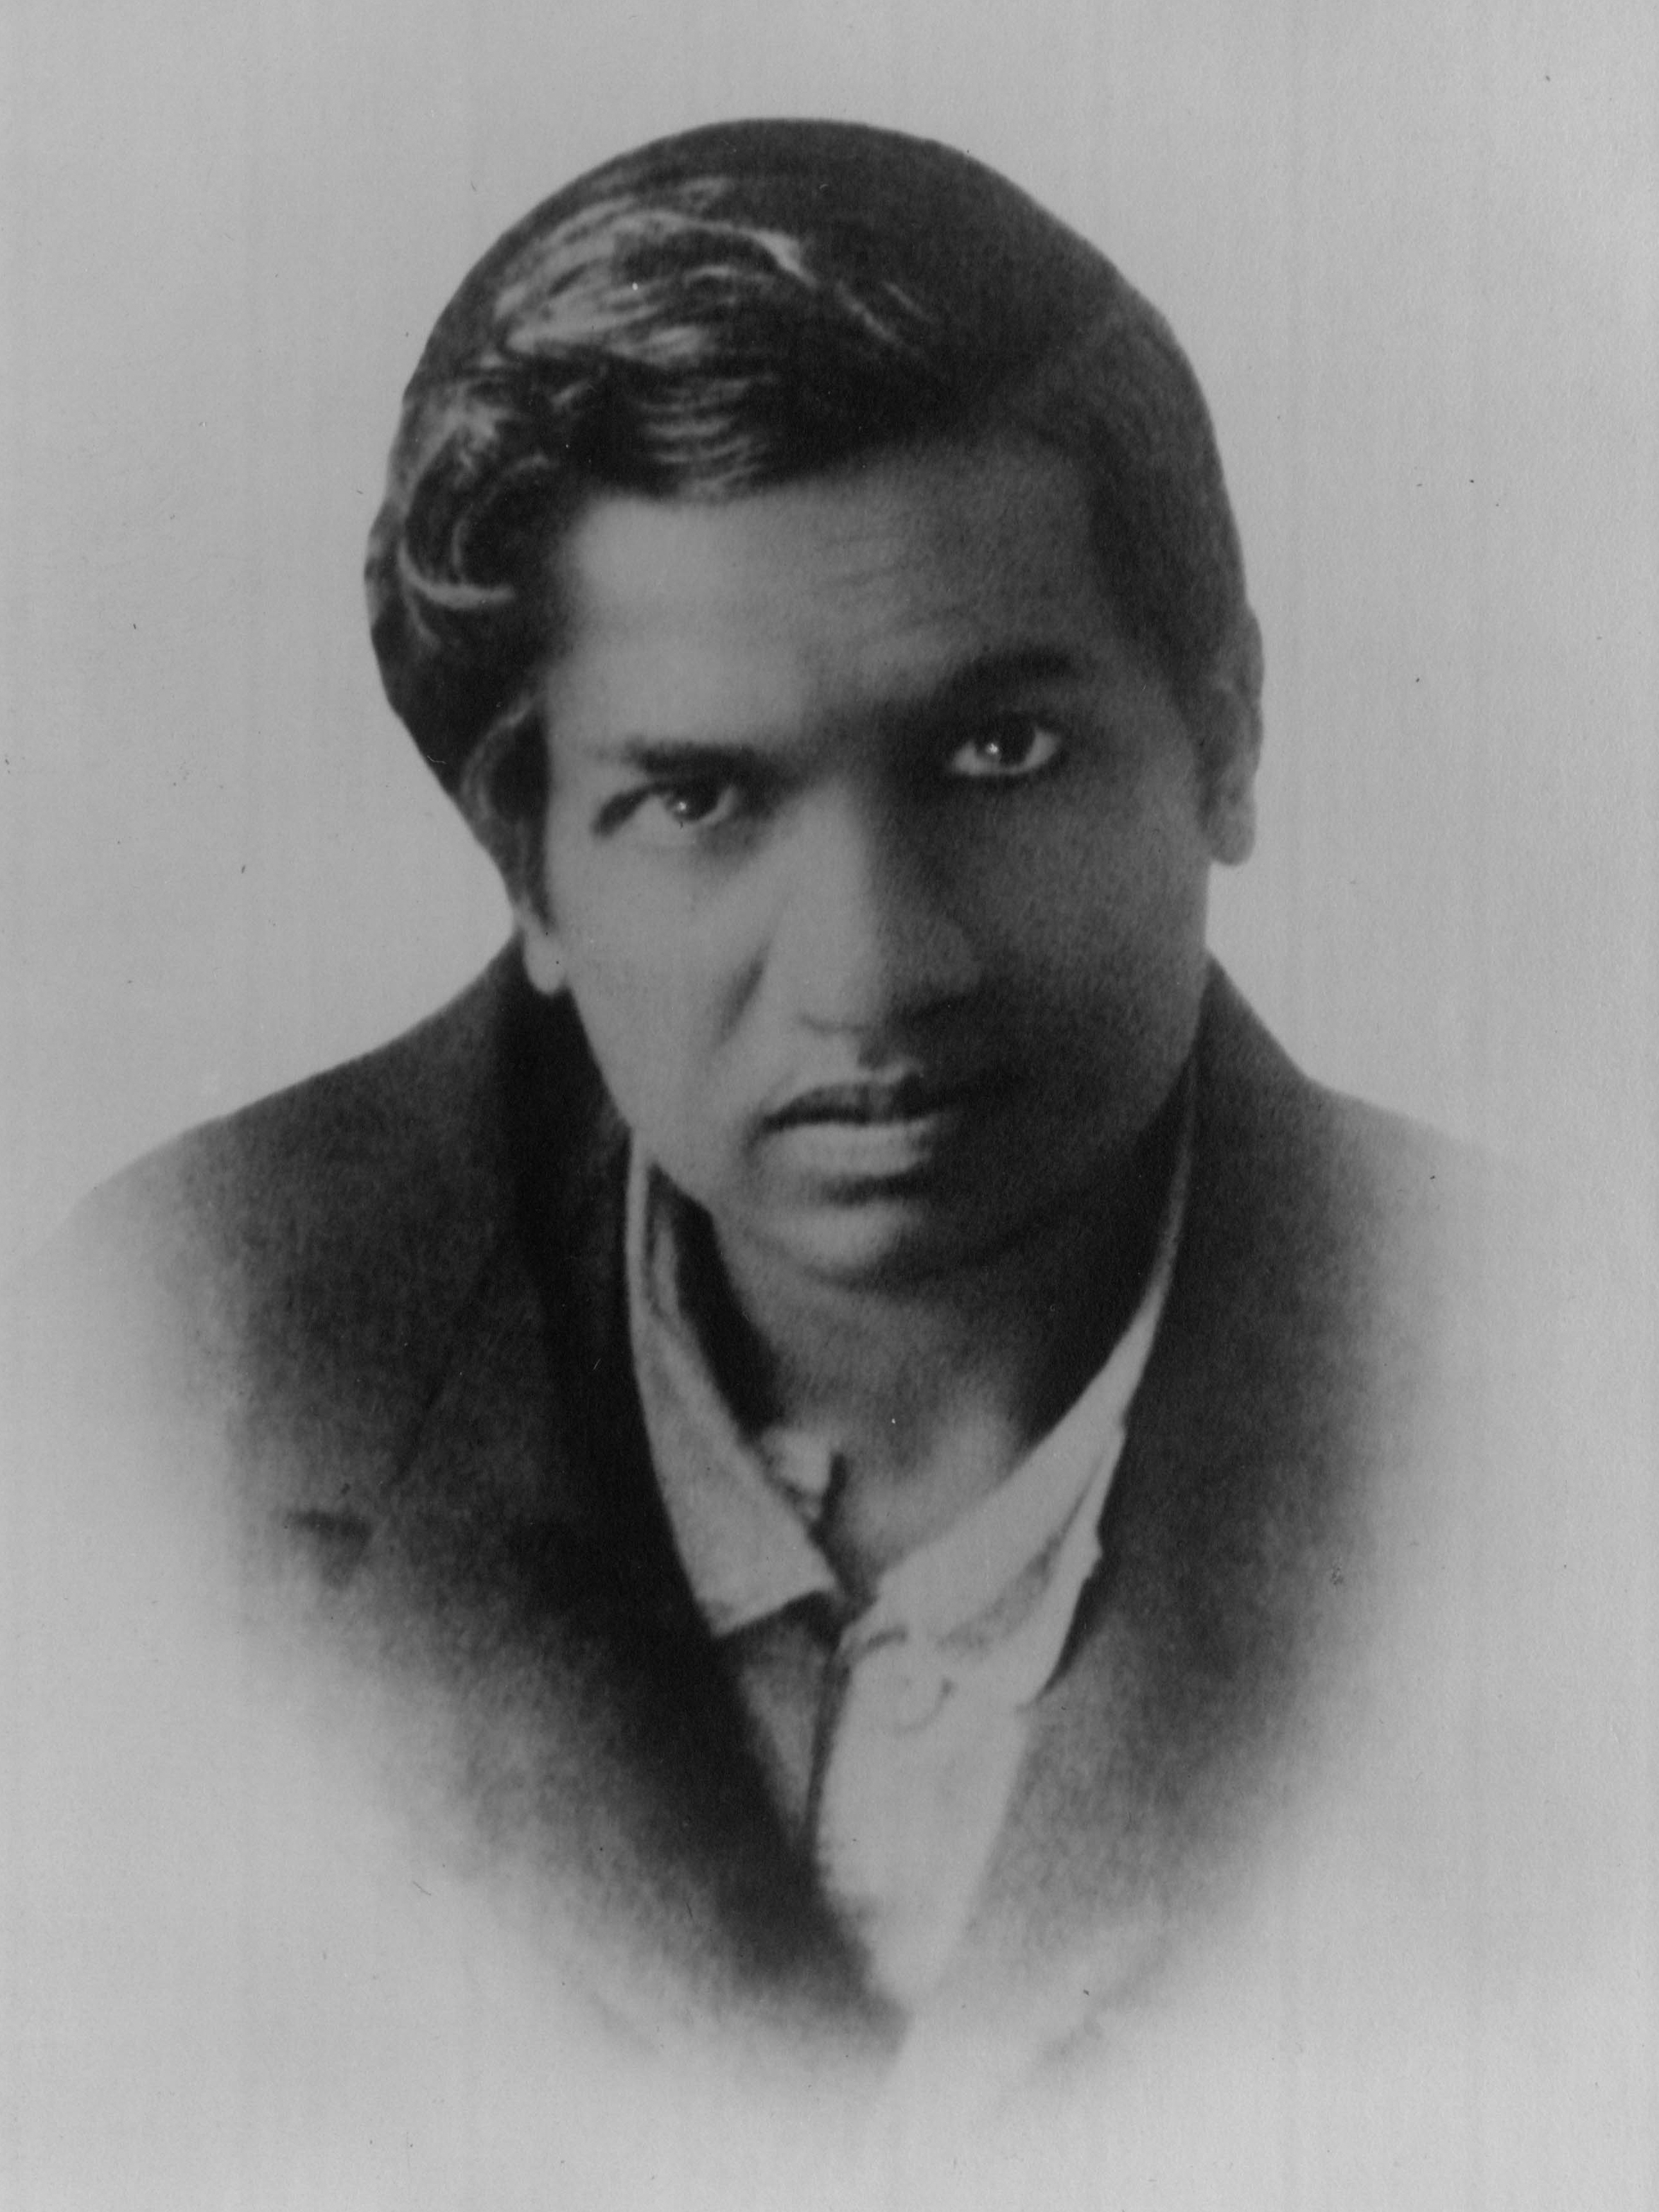
\includegraphics[scale=0.15]{photos/Ramanujan.jpg}
    %\\ \textbf{ {\footnotesize Passport photograph of } } \\ \textbf{ {\footnotesize Ramanujan created in 1913}}
%\end{figure}

First, recall the formula for geometric series 
$$1 + x + x^2 + x^3 + x^4 + ... = \frac{1}{1-x}$$
Notice that by differentiating on both sides as a function of $x$, we get
$$1 + 2x + 3x^2 + 4x^3 + ... = \frac{1}{(1-x)^2}$$
By plugging-in $x = -1$ in this formula, we get
\[1 - 2 + 3 - 4 + ... = \frac{1}{(1 + 1)^2} = \frac{1}{4}\tag*{(1)} \]
Now, define
$$c = 1 + 2 + 3 + 4 + ...$$
and notice that
\begin{align*}
    -3c &= c - 4c \\
    &= 1 + 2 + 3 + 4 + 5 + 6 +... \\
    & - ( \quad \; \, 4 \quad \ \ + 8 \quad \ \ + 12 + ... \ ) \\
    &= 1 - 2 + 3 -4 + 5 - 6 + ... \\
    &= \frac{1}{4}
\end{align*}
where the last step is due to equation (1). Solving for $c$ gives us
$$1 + 2 + 3 + 4 + ... = - \frac{1}{12}$$
This formula is quite surprising and obviously false. This precise example is now well-know in the mathematical culture because of its link with some more serious mathematics (the Riemann Zeta Function) and physics (the Casimir Effect). 

Another example of the same nature shows a similar obvious contradiction with the same manipulations. Consider
$$c = 1 + 2 + 3 + 4 + ...$$
and notice that
\begin{align*}
    0 &= c-c \\
    &= 1 + 2 + 3 + 4 + ... \\
    & - (0 + 1 + 2 + 3 + ...) \\
    &= (1 - 0) + (2 - 1) + (3 - 2) + (4 - 2) + ... \\
    &= 1 + 1 + 1 + 1 + ...
\end{align*}
which gives us
\[1 + 1 + 1 + 1 + ... = 0 \tag*{(2)}\]
Again, applying this same manipulation to equation (2) gives us 
\begin{align*}
    0 &= 0-0 \\
    &= 1 + 1 + 1 + 1 + ... \\
    & - (0 + 1 + 1 + 1 + ...) \\
    &= (1 - 0) + (1 - 1) + (1 - 1) + (1 - 1) + ... \\
    &= 1 + 0 + 0 + 0 + ...
\end{align*}
which is a contradiction since $0 \neq 1$. 

It turns out that every \textit{invalid} step in the two previous examples comes either from some problems with convergence or from the manipulation of series in the same way as finite sums. These problems are precisely what we made sure to go over precisely towards a rigorous proof. It is clear now that using the wrong notations or not making sure of convergence can potentialy and easily lead to some errors and contradictions. This shows why rigor is needed most of the time.

\subsection{Fourier's Theorem}

The Birth of Calculus (around the late 17th century) can be compared to an explosion in the field of Mathematics. In just a few decades, a whole new set of ideas, techniques, brand new results and mathematical geniuses appeared. However, looking back at some texts of this period clearly shows that the usual mathematical rigor that we know since Ancient Greece was left out of the party. A way of explaining why it was the case is the fact that in practice (in physics for example), everything seemed to work perfectly. Why spending a huge amount of time proving rigorously a formula if everyone knows that it works and everyone is already using it ? It turns out that this lack of rigor became more of an obstacle as time went by. To illustrate this point, it will be better to focus on a specific example.

%\begin{figure}[h]
    %\centering
    %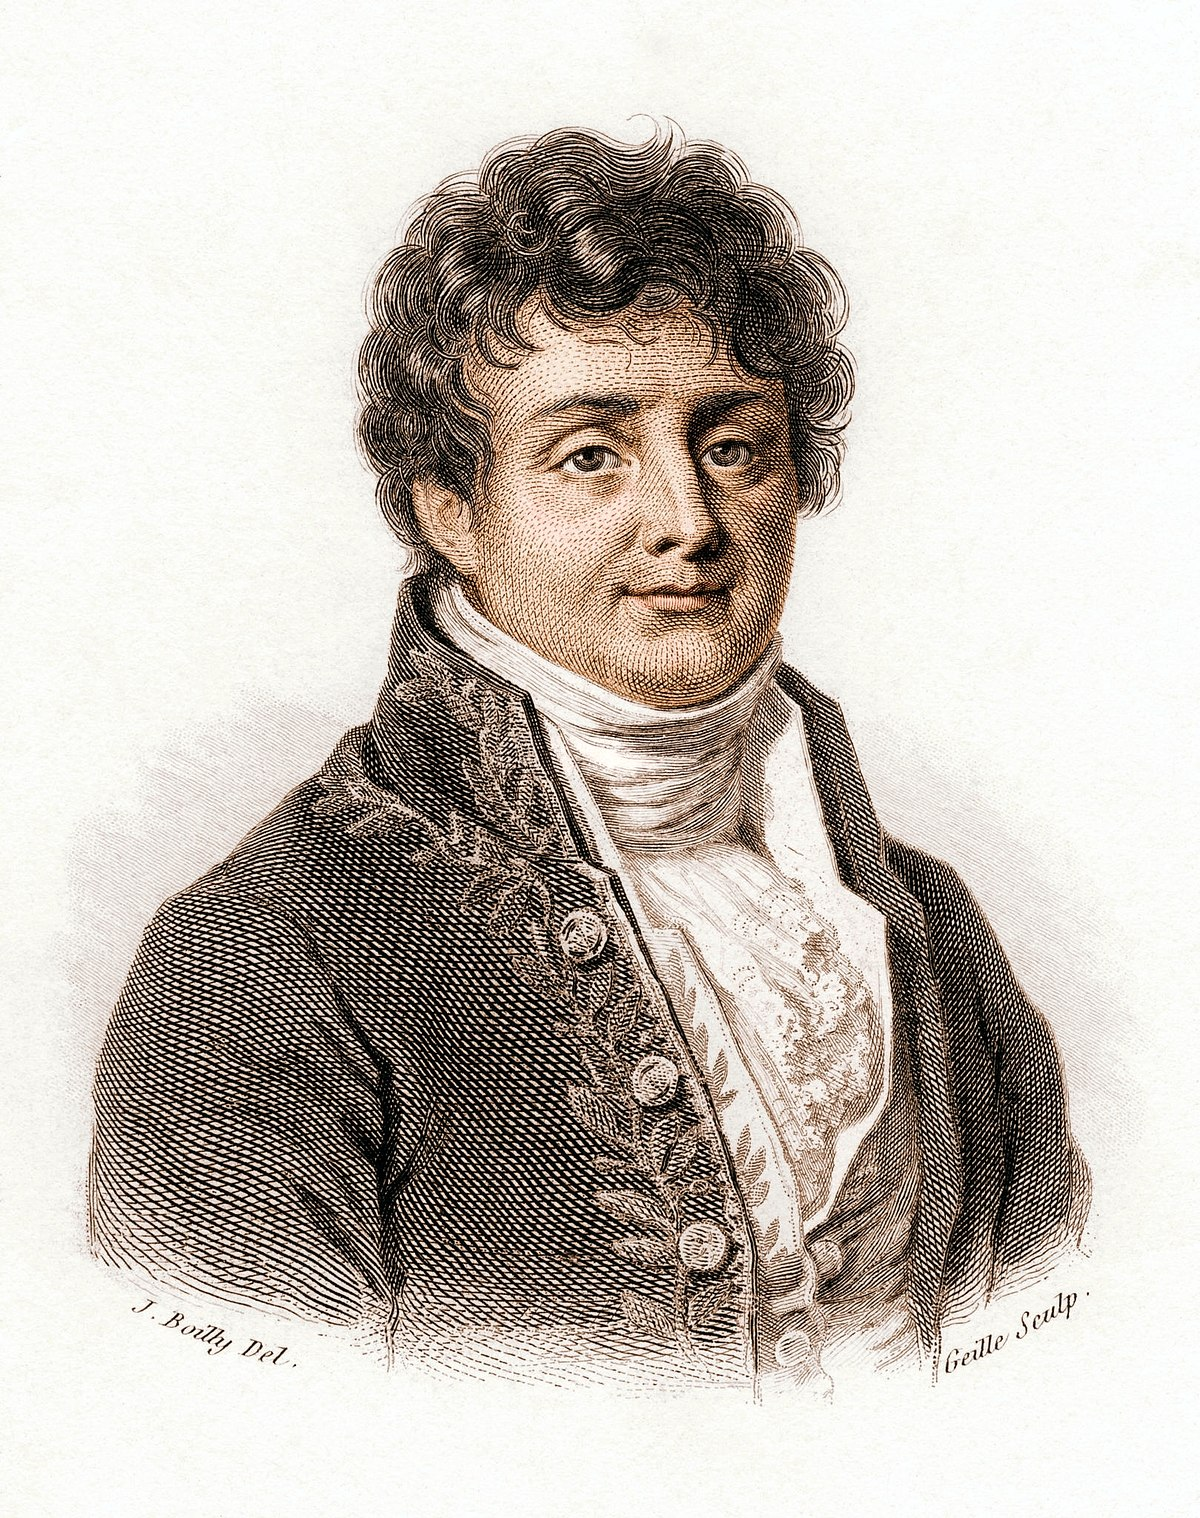
\includegraphics[scale=0.15]{photos/fourier.jpg}
    %\\ \textbf{ {\footnotesize Joseph Fourier } }
%\end{figure}

In the first half of the 19th century, Joseph Fourier published his work on the theory of heat propagation and the study of the Heat Equation using trigonometric series \cite{fourier1822}. It is in this period that he published what we now call Fourier's Theorem which basically states that any function can be represented as a trigonometric series (the details are not important here, even knowing what a trigonometric series is isn't important). However, Fourier didn't prove his theorem so most of his contemporaries tried to, such as Augustin Louis Cauchy, Siméon Denis Poisson and Peter Lejeune Dirichlet. It is only the latter that actually succeded in giving a rigorous enough and general enough proof of Fourier's Theorem (a version of it, not the full theorem). But to do so, he had to define the notion of function, even thought everyone knew what a function was for centuries.

A few decades later, another mathematician pursued Dirichlet's work on Fourier's Theorem: Bernhard Riemann. In the middle of the 19th century, Riemann tried to improve Dirichlet's proof but noticed that the notion of integral, as the concept of function before Dirichlet, wasn't well defined and needed a clear definition. Without a clear and formal definition of the integral, it would be hard to prove some theorems that involve taking an integral (such as Fourier's Theorem). This is the main motivation behind what we now call Riemann's Integral; which became the first widely accpeted rigorous definition of the integral. But again, everyone knew before Riemann what was an integral, Riemann didn't invent the integral.

Again, a few decades later, after a lot of progress on proving Fourier's Theorem, while working on a theorem related to Fourier's Theorem, the mathematician Georg Cantor found himself defining the notion of real numbers and even the premices of a modern theory of sets. This theory of sets became the foundations of modern mathamatics and is still an active field of research today. 

The question now is: why defining these intuitive notions after centuries of everyone knowing intuitively what they were? The answer is simple: it turned out that none of these notions were intuitive. What is a set ? A collection of objects ? But what is a collection then ? Similarly, what is an integral ? The area under the curve of a function ? But what is a function or even an area ? Today, we have whole branches of mathamatics dedicated to answering these questions: Measure Theory, Set Theory, Integration Theory, ... It is for this matter that the first step towards a rigorous proof was to define precisely the concepts mentionned in the claim of the theorem. Again, as for the previous section, we get here another reason why rigor is important: some intuitive notions may in fact not be intuitive at all and it is worth trying to understand why. For more details about Fourier's Theorem and its consequences on Mathematical Analysis, I wrote with Nisrine Sqalli a whole article on the subject : \textit{Fourier Analysis: The Catalyst of Modern Analysis} \cite{fourier}.

\section{Conclusion}

Intuition may be very important and very powerful but let's not forget that it is not perfect. Intuitively, the earth is flat and the sun revolves around the earth. With rigor, we end up asking seemingly simple questions that require creating completely new worlds that intuition would have never let us explore to answer the question. It is only by rigor that we were able to understand the true nature of Fourier's Theorem and many others. In conclusion, the goal here was to explain why the rigor in mathematics wasn't an obstacle but the exact opposit.

Concerning the proof of the Divergence of Harmonic Series, as I said at the beginning, I found it nowhere else on the internet or by asking some professors, so please, if you have heard of this proof from somewhere else than this paper, let me know by emailing me at samy.lahloukamal@mail.mcgill.ca so I can update this document. Thank you.

% REFERENCES
\newpage
\bibliographystyle{abbrv}
\bibliography{sources}

\end{document}